\documentclass{article}
\usepackage{amsmath}
\usepackage{amsfonts}
\usepackage{amssymb}
\usepackage{graphicx}
\usepackage{tikz}
\usepackage{pgfplots}
\pgfplotsset{compat=1.18}
\begin{document}

\section{TikZ Diagrams Examples}
This document demonstrates various TikZ diagrams that can be rendered in Overleaf. Each section shows different types of diagrams created using React components.


\section{Geometric Shapes}
This section demonstrates basic TikZ geometric shapes.

\begin{figure}[h]
\centering
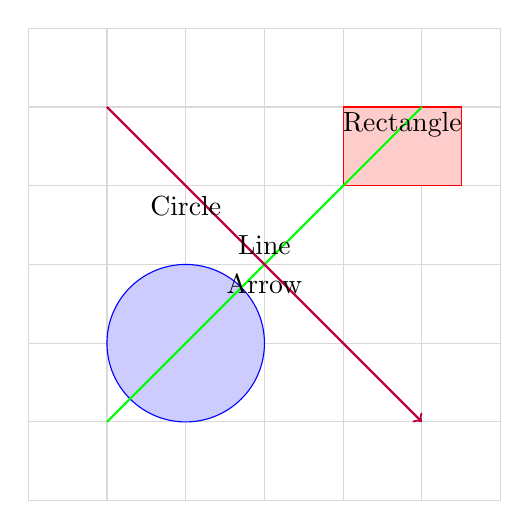
\begin{tikzpicture}[scale=1]
\draw[gray!30][step=1cm] (0,0) grid (6,6);
\draw[fill=blue!20, draw=blue] (2,2) circle (1cm);
\draw[fill=red!20, draw=red] (4,4) rectangle (5.5,5);
\draw[thick, green] (1,1) -- (5,5);
\draw[->, thick, purple] (1,5) -- (5,1);
\node[above] at (2,3.5) {Circle};
\node[above] at (4.75,4.5) {Rectangle};
\node[above] at (3,3) {Line};
\node[below] at (3,3) {Arrow};

\end{tikzpicture}
\end{figure}


\section{Flowchart Example}
This section shows a simple flowchart created with TikZ.

\begin{figure}[h]
\centering
\begin{tikzpicture}[scale=1]
\node[fill=green!20][circle, draw] at (0,0) {Start};
\node[fill=blue!20][rectangle, draw] at (0,-2) {Process};
\node[fill=yellow!20][diamond, draw] at (0,-4) {Decision};
\node[fill=green!20][rectangle, draw] at (3,-4) {Yes};
\node[fill=red!20][rectangle, draw] at (-3,-4) {No};
\node[fill=red!20][circle, draw] at (0,-6) {End};
\draw[->] (0,-0.5) -- (0,-1.5);
\draw[->] (0,-2.5) -- (0,-3.5);
\draw[->] (0.5,-4) -- (2.5,-4);
\draw[->] (-0.5,-4) -- (-2.5,-4);
\draw[->] (0,-4.5) -- (0,-5.5);

\end{tikzpicture}
\end{figure}


\section{Mathematical Diagram}
This section demonstrates a mathematical diagram with axes and functions.

\begin{figure}[h]
\centering
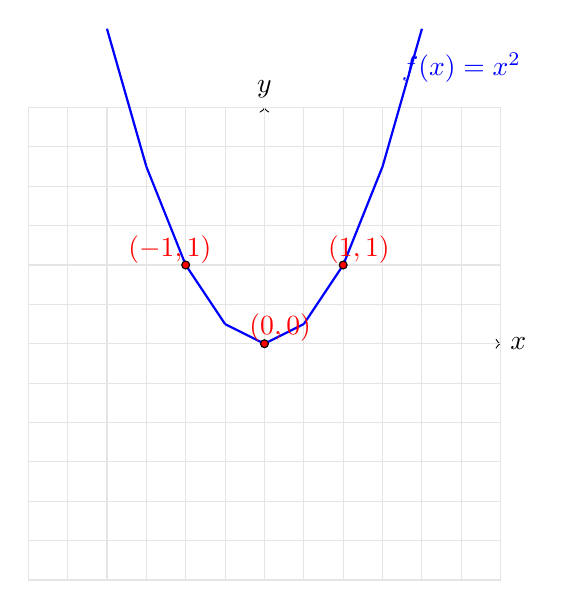
\begin{tikzpicture}[scale=1]
\draw [->] (-3,0) -- (3,0) node[right] {$x$};
\draw [->] (0,-3) -- (0,3) node[above] {$y$};
\draw[gray!20][step=0.5cm] (-3,-3) grid (3,3);
\draw[thick, blue] (-2,4) -- (-1.5,2.25);
\draw[thick, blue] (-1.5,2.25) -- (-1,1);
\draw[thick, blue] (-1,1) -- (-0.5,0.25);
\draw[thick, blue] (-0.5,0.25) -- (0,0);
\draw[thick, blue] (0,0) -- (0.5,0.25);
\draw[thick, blue] (0.5,0.25) -- (1,1);
\draw[thick, blue] (1,1) -- (1.5,2.25);
\draw[thick, blue] (1.5,2.25) -- (2,4);
\draw[fill=red] (0,0) circle (0.05cm);
\draw[fill=red] (1,1) circle (0.05cm);
\draw[fill=red] (-1,1) circle (0.05cm);
\node[blue] at (2.5,3.5) {$f(x) = x^2$};
\node[red] at (0.2,0.2) {$(0,0)$};
\node[red] at (1.2,1.2) {$(1,1)$};
\node[red] at (-1.2,1.2) {$(-1,1)$};

\end{tikzpicture}
\end{figure}


\section{Simple Circuit Diagram}
This section shows a simple electrical circuit diagram.

\begin{figure}[h]
\centering
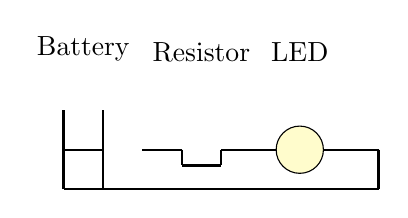
\begin{tikzpicture}[scale=1]
\draw[thick] (0,0) -- (0,1);
\draw[thick] (0.5,0) -- (0.5,1);
\draw[thick] (0,0.5) -- (0.5,0.5);
\draw[thick] (1,0.5) -- (1.5,0.5);
\draw[thick] (1.5,0.5) -- (1.5,0.3);
\draw[thick] (1.5,0.3) -- (2,0.3);
\draw[thick] (2,0.3) -- (2,0.5);
\draw[thick] (2,0.5) -- (2.5,0.5);
\draw[fill=yellow!20, draw=black] (3,0.5) circle (0.3cm);
\draw[thick] (2.5,0.5) -- (2.7,0.5);
\draw[thick] (3.3,0.5) -- (3.5,0.5);
\draw[thick] (3.5,0.5) -- (4,0.5);
\draw[thick] (4,0.5) -- (4,0);
\draw[thick] (4,0) -- (0,0);
\node[above] at (0.25,1.5) {Battery};
\node[above] at (1.75,1.5) {Resistor};
\node[above] at (3,1.5) {LED};

\end{tikzpicture}
\end{figure}




\end{document}